\chapter{Force Diagrams}
\label{ch:ForceDiagram}
The wing box shall be designed such that it can withstand the wing loads by providing sufficient stiffness. This Chapter will analyze the forces and moments acting on the wing and produce clear graphs of their variation along the structure. \autoref{sec:fd_modeling_approach_and_assumptions} states all simplifications and assumptions made for the wing model. The aerodynamic loading is then derived in \autoref{sec:fd_aerodynamic_loading_analysis} using XFLR5 simulations based on the wing geometry established in \textit{Wing Aerodynamic Design} \cite{Koppejan2024WingDesign}. Diagrams of the shear force, bending moment and torque are constructed in \autoref{sec:fd_shear_moment_torque}. The most critical cases are presented and analyzed separately in \autoref{sec:fd_critical_cases}.

\section{Modeling Approach and Assumptions} \label{sec:fd_modeling_approach_and_assumptions}
%A list of assumptions made in the derivation of the axial force, shear force, bending moment and torque diagrams.

The aim of this report is to provide a \textit{preliminary} design of the wing. Therefore, several assumptions are made regarding the wing and loads to simplify the loading problem. This section describes the reasons for these steps, their validity and the consequences they have on the results of the analysis.

\subsection*{Coordinate System}
% Note that the transformation to the tangential force component is not required for this assignment. (small angle of attack)
In the interest of avoiding confusion, it is important to define a suitable coordinate system. The XFLR5 simulations provide results in the \textit{body reference frame}, while the stiffness calculations are evaluated and graphically described for the \textit{aerodynamic reference frame} \cite{Timmer2024ProjectDesign}.\\

\noindent The transformation of the lift and drag per unit span ($L'$ and $D'$, respectively) from the aerodynamic reference frame into a normal force $N'$ (see: \autoref{fig:forces_coordinate_transformation} \cite{Timmer2024ProjectDesign}) in the body reference frame can be done according to \autoref{eq:forces_normal_transformation} \cite{Timmer2024ProjectDesign}, \\

\begin{equation}    \label{eq:forces_normal_transformation}
    N'(y)=cos(\alpha)L'(y)+sin(\alpha)D'(y)
\end{equation}

\begin{figure}[H]
    \centering
    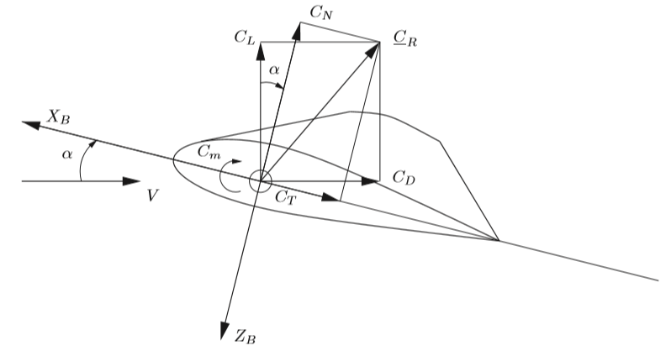
\includegraphics[width=0.5\linewidth]{figures/coordinates_converting_forces.png}
    \caption{Converting Aerodynamic Forces to Body Forces \cite{Timmer2024ProjectDesign}}
    \label{fig:forces_coordinate_transformation}
\end{figure}


\noindent where $\alpha$ is the angle of attack. Note that for small values of $\alpha$, the normal force is approximately equal to the aerodynamic lift.\\

\noindent A simplified visualization of the wing loading, as well as the coordinate system used for the calculation of the shear, bending and torsion, is showcased in \autoref{fig:candidate_coordinate_system}. For the purposes of this analysis, A distributed force $w(x)$ will be considered, as well as the engine weight $P_E$, located at $x_E$, and its corresponding bending moment $M_E$.

\begin{figure}[H]
    \centering
    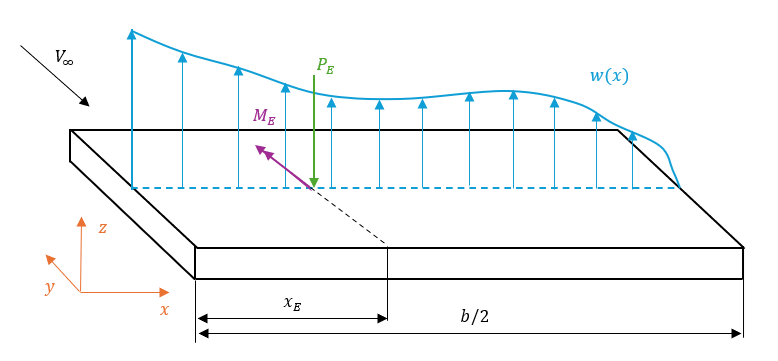
\includegraphics[width=0.5\linewidth]{beam_loading.png}
    \caption{Wing Loading Visualization}
    \label{fig:candidate_coordinate_system}
\end{figure}


\subsection*{Wing Sweep}
The planform design established in \textit{Wing Aerodynamic Design} \cite{Koppejan2024WingDesign} features a swept wing. Swept wings introduce complex load phenomena into the structure, which are outside of the scope of this course \cite{Timmer2024AE2111-IReader}. Therefore, a simpler shape will be considered for the construction of force and moment diagrams - an equivalent trapezoidal wing with a constant sweep angle (see: \autoref{fig:fd_assumptions_equivalent_unswept_wing}). The new model can be assumed to have the same values as the original wing, with the exception of the sweep at the flexural axis, which is reduced from the original sweep angle $\Lambda$ to zero \cite{Timmer2024AE2111-IReader}.
\begin{figure}[h]
    \centering
    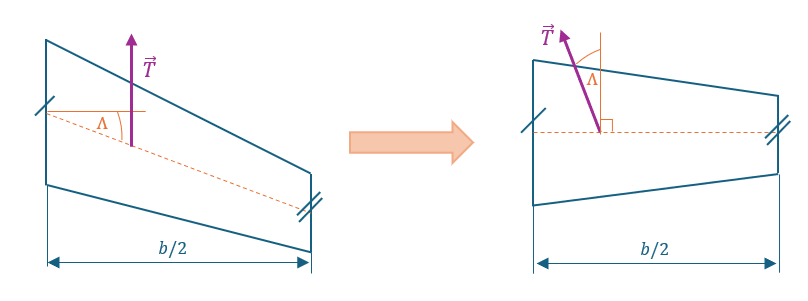
\includegraphics[width=0.85\linewidth]{figures/wing_sweep_effect.png}
    \caption{Equivalent unswept wing model}
    \label{fig:fd_assumptions_equivalent_unswept_wing}
\end{figure}

\noindent One consequence of this assumption is the changed direction of the thrust - as shown in \autoref{fig:fd_assumptions_equivalent_unswept_wing}, the orientation of the vector changes by an angle $\Lambda$. This happens because of the nature of the simplification - the whole planform is rotated to negate the effect of the sweep, and so is the thrust vector \cite{Timmer2024AE2111-IReader}.\\

\noindent The use of an equivalent trapezoidal wing is valid for modelling the variation of aerodynamic forces across the wing. However, it cannot be used in XFLR5 simulations, as the wing sweep affects the lift distribution, resulting in an overestimation of lift force towards the base of the wing, and an underestimation at the tips compared to the swept wing \cite{Timmer2024AE2111-IReader}.

\subsection*{In-Plane Forces and Moments}
The simplified loading case only considers shear forces in the vertical direction, i. e. perpendicular to the chord line. Therefore, the in-plane shear acting in the direction tangential to the chord line will be neglected. The same applies to bending moments - only those acting along the axis normal to the chord line are analyzed, and the in-plane bending of the wing box will not be regarded.\\

\noindent Neglecting the in-plane loads will, indispensably, lead to an overestimation of the performance of the wingbox in terms of strength and stiffness. In-plane interferences may lead to structural fatigue and shear fractures in metals \cite{Yin2015AMaterials}. However, the contribution of these loads to the shear, bending and torsion of the wingbox is negligible \cite{Timmer2024AE2111-IReader}, and hence, they are not considered in this part of the structural analysis.











%Note that formally speaking, point forces and couple moments can also be included in the distributed loading functions by use of Dirac-delta functions. However, for sake of simplicity, point forces and couple moments will be treated separately from the distributed load



\section{Aerodynamic Loading Analysis}  \label{sec:fd_aerodynamic_loading_analysis}
%Comment on the different reference frames for XFLR5 and force analysis [Fig. 9, p. 26 of the Reader].


\section{Shear Force, Bending Moment, and Torque}   \label{sec:fd_shear_moment_torque}
%Derivation of the shear force, bending moment and torque diagrams, and the corresponding plots. 

%Include two graphs for each plot: one corresponding to a critical load case with positive load factor found in WP4.3, and one corresponding to a critical load case with negative load factor found in WP4.3. Note that the inertial force on all elements depends on the load factor.
This section focuses on the formulae derivation and graphical representation of the shear force, bending moment, and torque acting on the wingbox. These are determined by the distributed aerodynamic loading, previously obtained in \autoref{sec:fd_aerodynamic_loading_analysis}.

\subsection*{Shear Force}
%shear force specific assumption
\noindent Adding to the general assumptions made above, the calculation of the shear force along the wing will only include the shear force contribution due to the lift distribution and none of the external force such as engine weight, fuel weight, and the weight of the wing itself. This assumption is deemed to be valid as it will cause a conservative estimation of the shear force. The shear force can be expressed in terms of the distributed loading as shown in \autoref{eq:shear_force_relation}

\begin{equation} \label{eq:shear_force_relation}
    w(x) = -\frac{dV}{dx}
\end{equation}
\noindent This expression can be integrated to obtain an expression for the shear force distribution along the wing as shown in \autoref{shear_force_integral}
\begin{equation} \label{shear_force_integral}
    V(x) = \int^L_x{w(x)dx}
\end{equation}

\subsection*{Bending Moment}
The bending moment $M$ is generally expressed as the second integral of the distributed load function, and hence closely related to the shear force $V$. It can be calculated by integrating \autoref{eq:fd:moment_shear_relation} \cite{Timmer2024AE2111-IReader} along the \textit{x}-axis.
\begin{equation}    \label{eq:fd:moment_shear_relation}
    V(x)=\frac{dM}{dx}
\end{equation}

\begin{comment}
Suppose a couple moment $M$ is applied at a location $x_2$ \todo{Would do nicely with a figure}. The bending moment at a given spanwise location $x$ can be expressed using \autoref{eq:fd_moment_at_x} \cite{Timmer2024AE2111-IReader}.
\begin{equation}    \label{eq:fd_moment_at_x}
   -M(x)=\int^L_x{V(x)dx}\space+M\left(1-u_{x_2}(x)\right)
\end{equation}
\noindent In this case, $u_{x_2}$ is the step function which attains a value of $0$ for $x<x_2$ and $1$ for $x\geq x_2$. In the case of an aircraft wing, a point moment would be a simplified representation of the bending relief provided by the engine weight $M_E$. The moment itself can be calculated as a product of the engine's weight $P_E$ and spanwise position $x_E$, i.e.:
\begin{equation*}
    M_E=P_E\cdot x_E
\end{equation*}

with $P_E$ and $x_E$ attaining the values of $(9630\cdot9.81)$ N and $9.37$ m, respectively, based on the results of propulsion system sizing from \textit{Further Aircraft Design} \cite{} \todo{cite WP3}. Substituting these values yields an engine bending relief moment $M_E$ of $885.187$ kNm.\\
\end{comment}
\noindent Since only the bending contributions of lift and engine weight are considered to act on the wing, and no additional bending moments are present in the load model, the internal bending moment $M$ at a given spanwise location $x$ can simply be evaluated as:
\begin{equation*}
    -M(x)=\int^{b/2}_x V(x)dx.
\end{equation*}



\subsection*{Torque}
% You may assume the shear centre to coincide with the centroid of the wing box cross section
For the torque, the shear center is required. Here, it can be assumed that the shear center coincides with the centroid of the wing box \cite{Timmer2024AE2111-IReader}, which is to be determined in \autoref{} \todo{cite section}. The loads of interest for the torque distribution are the lift distribution and the thrust force. The direction of the thrust force is pointed inward towards the fuselage as shown in \autoref{fig:fd_assumptions_equivalent_unswept_wing}. Therefore, to determine the torque, only the component of the thrust perpendicular to the shear center should be taken into account, using \autoref{fig:thrust_perpendicular}. 

\begin{equation}
    \label{fig:thrust_perpendicular}
    T_{\perp sc} = T\cos(\Lambda)
\end{equation}

\noindent The torsion at a location $x$ along the wing span can be determined using \autoref{eq:torsional_distribution}. In this equation, $L(x)$ is the function describing the distributed lift in the spanwise direction, $d(x)$ is the distance between the point of application of the distributed load and the shear centre, $d_1$ is the perpendicular distance between the orthogonal component of the thrust force T and the shear centre and $d_2$ is the distance between the application of the engine weight $W_E$ and the shear centre. $T_{\perp sc}$ is applied at position $x_1$, where the step function $u_{x_1}$ is equal to 0 for $x<x_1$ and 1 for $x\geq x_1$. $u_{x_2}$ behaves similar to this with the engine weight at $x_2$.

\begin{equation}
    \tau(x) = \int_x^{b/2}[L(x)d(x)]dx + T_{\perp sc}d_1 \left(1 - u_{x_1}(x) \right) - W_Ed_2\left(1 - u_{x_2}(x) \right)
    \label{eq:torsional_distribution}
\end{equation}

\noindent For the contribution of the weight of the engine to the internal torque distribution, the assumption is made that this load acts as a point force at the leading edge of the wing. This means that the distance $d_2$ is equal to the distance between the leading edge of the wing and the shear centre at the location $x_2$ along the shear centre. The engines are placed at $x_2 = 9.37$ m from the centre of the fuselage. The engine mass is equal to $9630$ kg. \\

\noindent The vertical distance between the shear centre and engine thrust is equal to $d_1$ and is to be determined when the centroid of the wing box is known. The spanwise location of the applied thrust is the same as for the weight of the engine and thus $x_1 = x_2 = 9.37$ m. The engine thrust is equal to $467.06$ kN. The sweep angle that is used in this equation is the half-chord sweep angle and is equal to $26.55$ deg.

\begin{equation}
    \tau(x) = \int_x^{31.36}[L(x)d(x)]dx + 467060 \cdot \cos{(26.55)} \cdot d_1 \left(1 - u_{9.37}(x) \right) - 9630 \cdot 9.81 \cdot d_2\left(1 - u_{9.37}(x) \right)
    \label{eq:torsional_distribution_with_numbers}
\end{equation}

\section{Explanation of Critical Cases} \label{sec:fd_critical_cases}
% Justification on why these load cases can be considered as the most critical